\begin{frame}{{\color{violet}IVs: Information Diversity \& {\color{salmon}Novelty} -- Ego}}

  \begin{columns}

    \begin{column}{0.5\linewidth}
      \begin{itemize}
        \item Topic Vectors by Keyword
        \item Keyword Selection: $k$-means Clustering of topics
        \item Information Diversity (${ID}_i$)
        \item {\color{salmon}Non-Redundant} Information (${NRI}_i$): ${ID}_i$ times total incoming e-mail 
      \end{itemize}
    \end{column}

    \begin{column}{0.5\linewidth}
      \begin{figure}
        \centering
        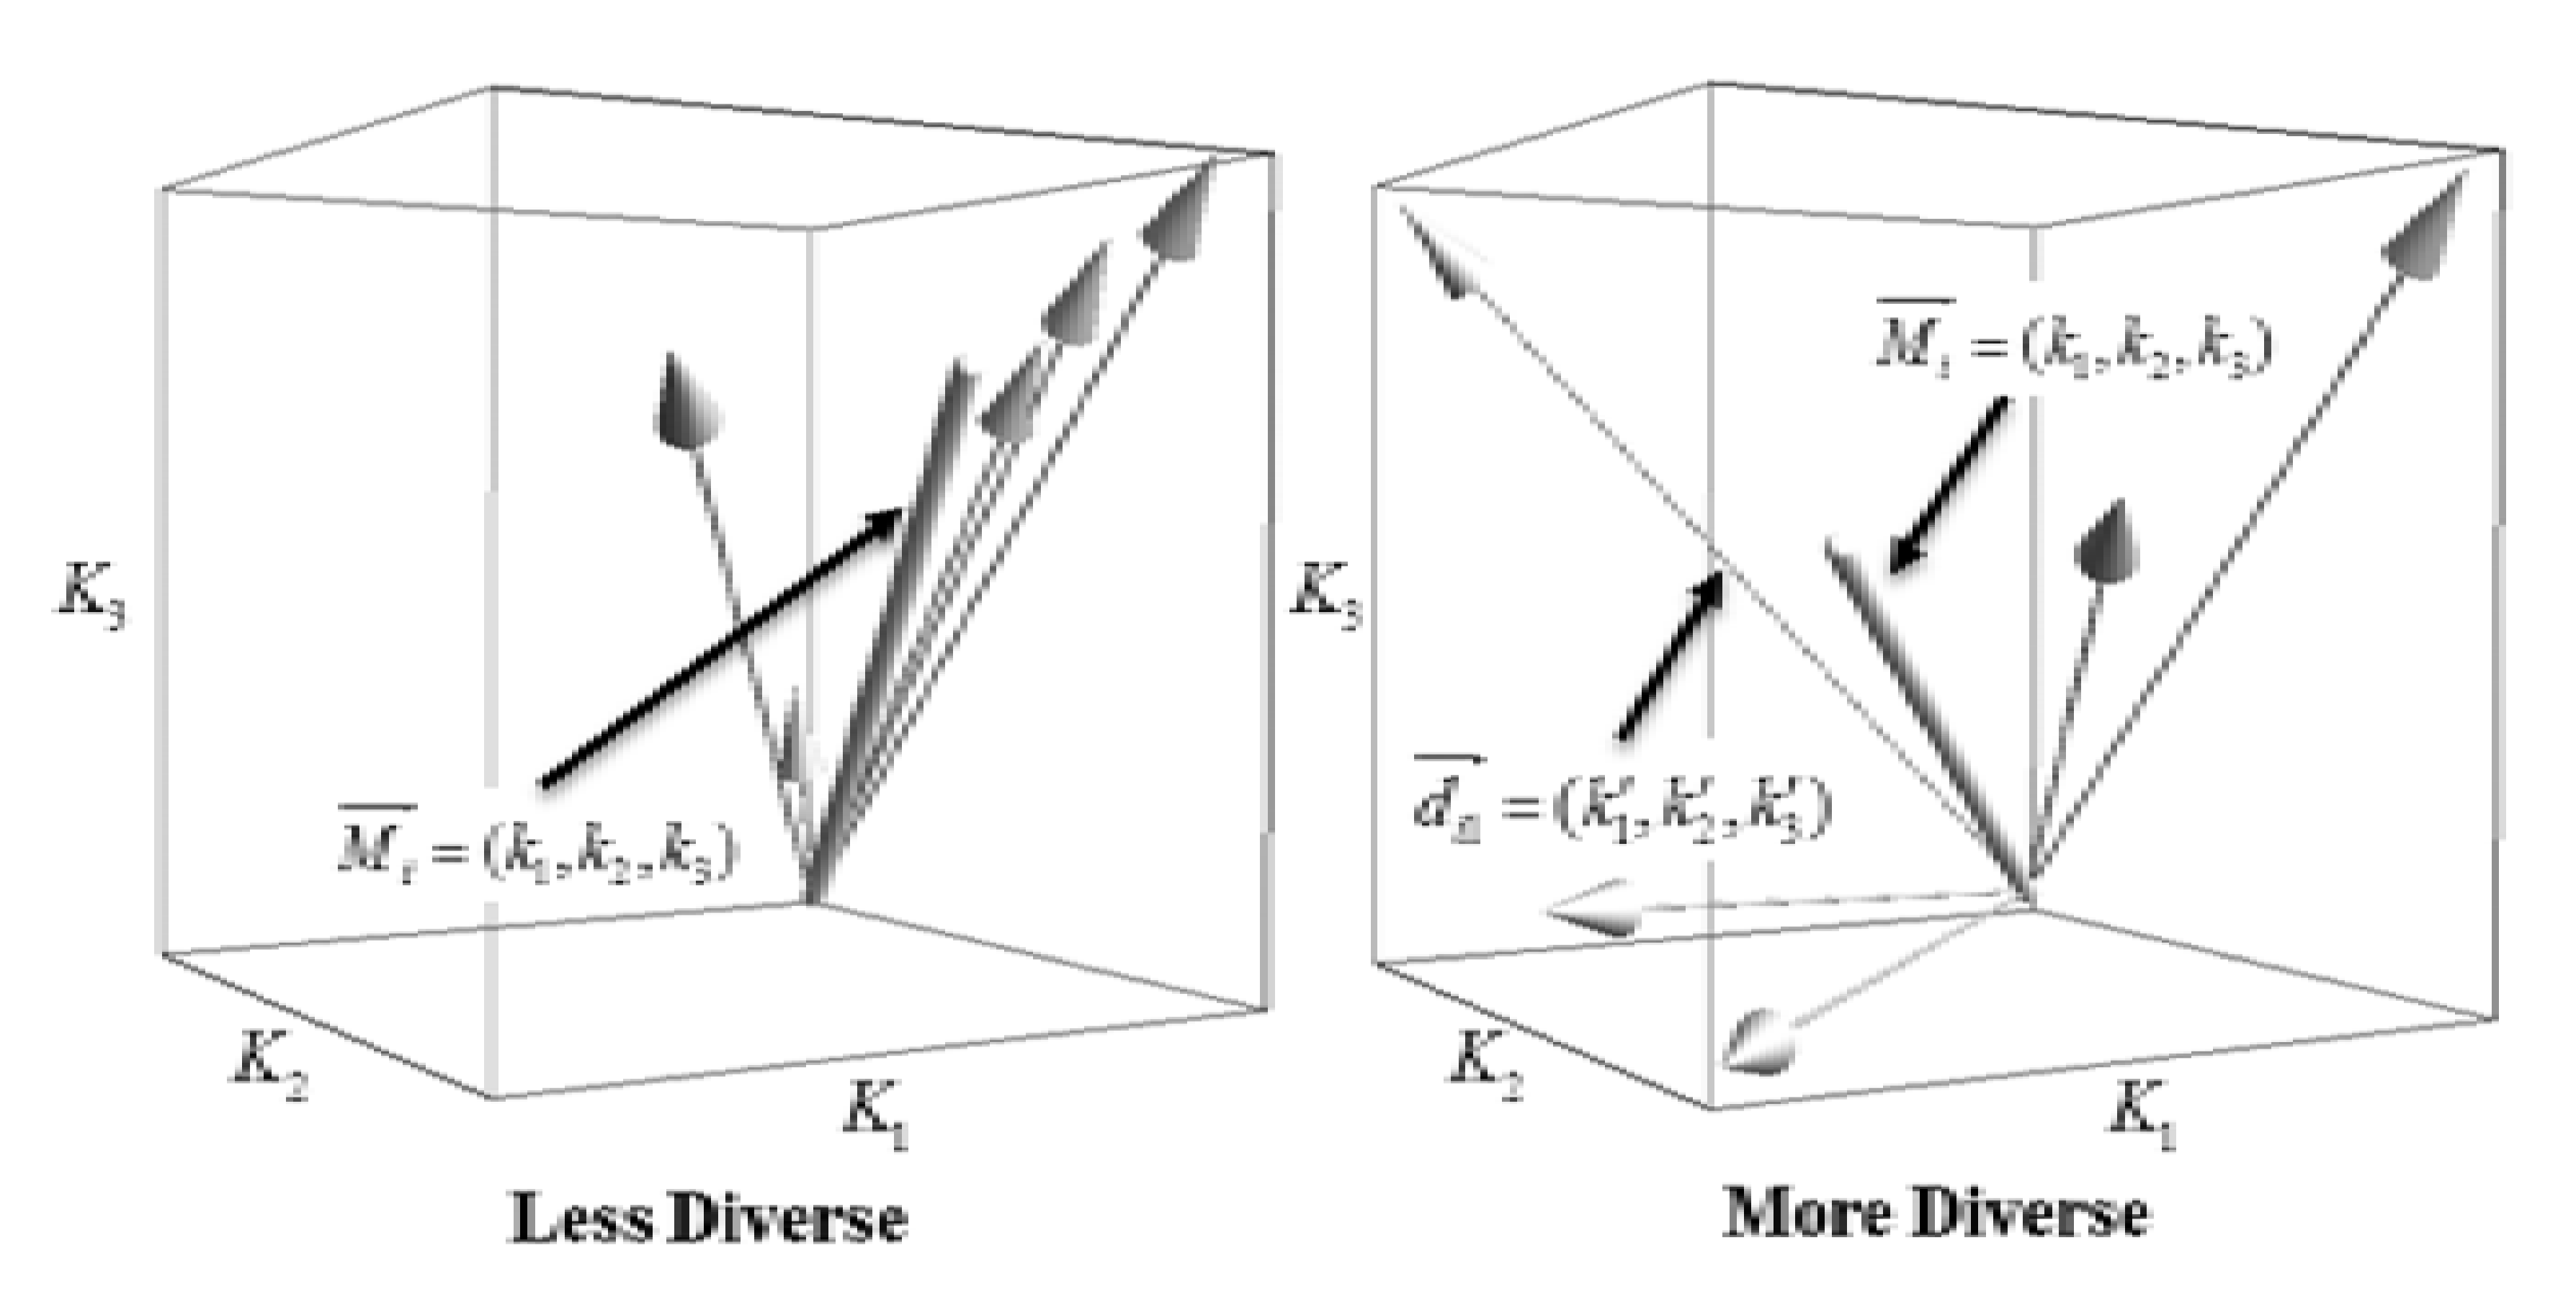
\includegraphics[width=\linewidth]{cos-dist2.png}
        % \caption{Cosine Distance}
      \end{figure}
      $${CosDist}_{ij} = 1 - Cos(d_{ij},M_{i})$$
      $${ID}_{i} = \frac{{\sum_{j=1}^{N} {CosDist}_{j}}^2}{N}$$
    \end{column}
    
  \end{columns}

  \note{
    k-means: High-frequency words in topics that maximize inter-topic coefficient of variation \& minimize intra-topic mean frequency variation.  
    ID: Avg. \underline{cosine distance} from \underline{cluster mean vector}
  }

\end{frame}
